\begin{solution}

\begin{enumerate}
\item The code listed below produces the desired plots.
(We use \verb|subplot| rather than superimposing the plots,
and we also include $N=4$ for the sake of comparison.)

[On the error plot, we include a line showing the rate of convergence
if the error was reduced exactly like $h^2$.  We see that the rates
(that is, the slope of the true error curve (solid) and this $h^2$
curve (dashed)) are quite close.  The follows from the fact that
our approximation to the second derivative makes an error of size
$h^2$; see the note for lectures~5 and~6.]



{\footnotesize\begin{verbatim}
 Nvec = [4 8 16 32 64 128];
 err = zeros(size(Nvec)); 
 figure(1), clf
 for j=1:length(Nvec)
    N = Nvec(j);
    h = 1/(N+1);
    x = h*[1:N]'; 
    A = (-2*eye(N)+diag(ones(N-1,1),1)+diag(ones(N-1,1),-1))/(h^2);
    f = 25*pi^2*cos(5*pi*x);
    u = A\f;
% plot the function, adding in the homogeneous values at the boundary;
% this tacks on extra entries for the x and u vectors:
    figure(1), subplot(3,2,j)
    plot([0;x;1],[0;u;0],'k-','linewidth',2), hold on
    axis([0 1 -2.5 2.5])
    xlabel('x')
    ylabel('u(x)')
    text(.05,-2.05,sprintf('N = %d',N))
% compute error
    true_u = 1-2*x-cos(5*pi*x);
    err(j) = max(abs(true_u - u));
 end
 print -depsc2 diffmats_a1.eps

% error plot
 figure(2), clf
 loglog(Nvec, err, 'k.-','linewidth',1.5), hold on
 loglog(Nvec, Nvec.^(-2), 'k--', 'linewidth',1.5)
 legend('Error', 'perfect h^2 convergence',1)
 loglog(Nvec, err, 'k.','markersize',20)
 set(gca,'fontsize',14)
 xlabel('N')
 ylabel('maximum error')
 title('Error in Approximate Solutions of the Homogeneous Dirichlet Problem')
 print -depsc2 diffmats_a2.eps
\end{verbatim}}

\begin{center}
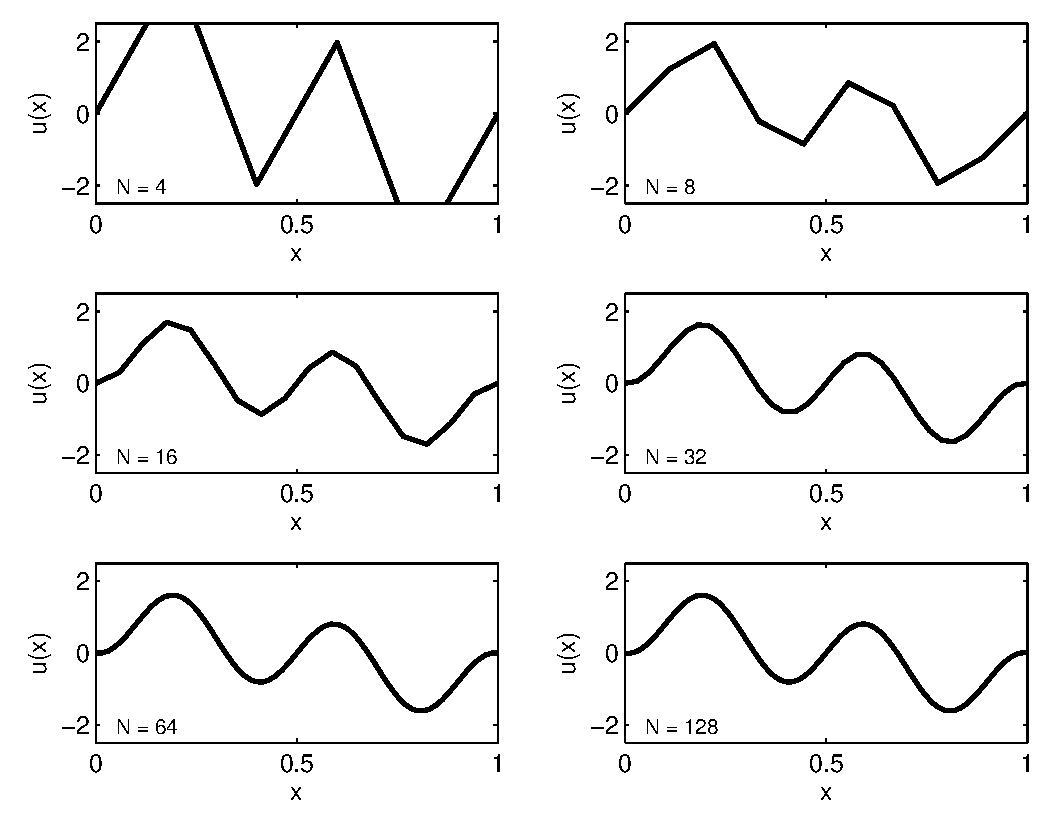
\includegraphics[scale=0.7]{diffmats_a1}
\end{center}
\begin{center}
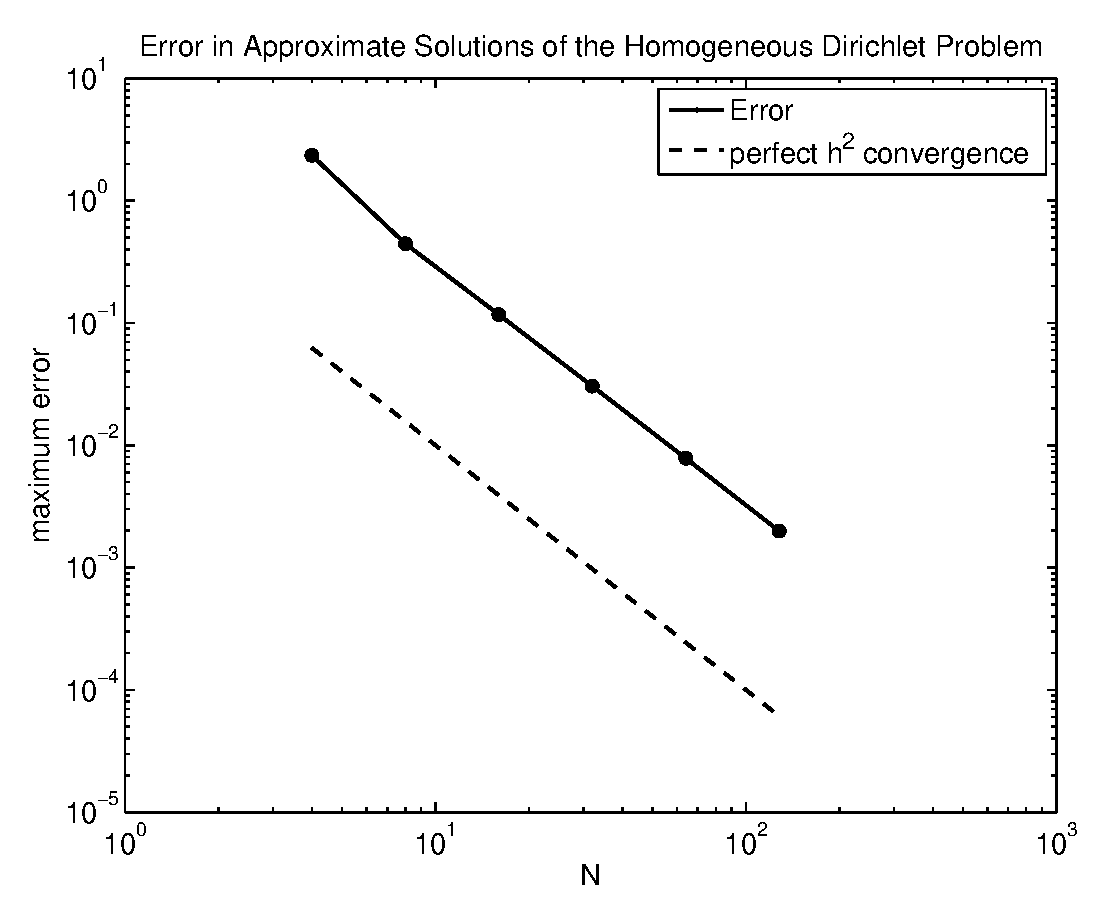
\includegraphics[scale=0.5]{diffmats_a2}
\end{center}

\item To impose inhomogeneous boundary conditions, we must make
      a correction to the right hand side vector to account for
      the fact that $u(0)$ and $u(1)$ are nonzero.  
      For example, when $N=3$ we have the equation
         \[ {1\over h^2} \bmatrix{1 &-2 & 1 & 0 & 0 \cr
                                     0 & 1 &-2 & 1 & 0 \cr
                                     0 & 0 & 1 &-2 & 1}
                      \bmatrix{u(0) \cr u(x_1) \cr u(x_2) \cr u(x_3) \cr u(1)}
             \approx 
             \bmatrix{u''(x_1) \cr u''(x_2) \cr u''(x_3)}
           = \bmatrix{f(x_1) \cr f(x_2) \cr f(x_3)}.\] 
       Suppose we have $u(0) = \alpha$ and $u(1) = \beta$.  
       Then we can write the above approximation in the form
       \[     {1\over h^2} \bmatrix{1 \cr 0 \cr 0} \alpha 
           +
               {1\over h^2} \bmatrix{-2 & 1 & 0  \cr
                                      1 &-2 & 1  \cr
                                      0 & 1 &-2 }
                            \bmatrix{u(x_1) \cr u(x_2) \cr u(x_3)}
           +   {1\over h^2} \bmatrix{0 \cr 0 \cr 1} \beta
             \approx 
        \bmatrix{f(x_1) \cr f(x_2) \cr f(x_3)}.\]
       Moving the two known vectors on the left to the right hand side,
       we obtain
       \[      {1\over h^2} \bmatrix{-2 & 1 & 0  \cr
                                      1 &-2 & 1  \cr
                                      0 & 1 &-2 }
                            \bmatrix{u(x_1) \cr u(x_2) \cr u(x_3)}
           \approx 
                 \bmatrix{f(x_1)-\alpha/h^2 \cr f(x_2) \cr f(x_3)-\beta/h^2}.\]
       The formula generalizes to larger values of $N$:  One imposes
       inhomogeneous Dirichlet boundary conditions by modifying the
       first and last entries of the right-hand side vector.

       [\textbf{GRADERS}: It is also possible to impose 
        inhomogeneous Dirichlet boundary conditions 
        for this problem by adding an appropriate line to the solution 
        from part~(a).  Please give credit for this solution, though
        I prefer the approach outlined here because it more easily
        generalizes to a broader class of operators.]

        The code below produces the requested plots, plus a few extra.

{\footnotesize \begin{verbatim}
 Nvec = [4 8 16 32 64 128];
 u0 = 1;
 u1 = 2;
 figure(1), clf
 for j=1:length(Nvec)
    N = Nvec(j);
    h = 1/(N+1);
    x = h*[1:N]'; 
    A = (-2*eye(N)+diag(ones(N-1,1),1)+diag(ones(N-1,1),-1))/(h^2);
    f = 25*pi^2*cos(5*pi*x);
    f(1) = f(1)-u0/(h^2);
    f(N) = f(N)-u1/(h^2);
    u = A\f;
% plot the function, adding in the inhomogeneous values at the boundary;
% this tacks on extra entries for the x and u vectors:
    subplot(3,2,j)
    plot([0;x;1],[u0;u;u1],'k-','linewidth',2), hold on
    axis([0 1 0 3.5])
    xlabel('x')
    ylabel('u(x)')
    set(gca,'ytick',[0:1:3])
    text(.05,.35,sprintf('N = %d',N))
 end
 print -depsc2 diffmats_b
\end{verbatim}} 

\begin{center}
\includegraphics[scale=0.7]{diffmats_b}
\end{center}

\item The mixed boundary conditions impose a further complication,
      as now we do not know a value for $u(1) = u(x_{N+1})$.
      Suppose that $u(0) = \alpha$.
      Again resorting to the $N=3$ case for illustrative purposes,
      we have
         \[ {1\over h^2} \bmatrix{1 &-2 & 1 & 0 & 0 \cr
                                     0 & 1 &-2 & 1 & 0 \cr
                                     0 & 0 & 1 &-2 & 1}
                      \bmatrix{\alpha \cr u(x_1) \cr u(x_2) \cr u(x_3) \cr u(x_4)}
             \approx 
             \bmatrix{u''(x_1) \cr u''(x_2) \cr u''(x_3)}
           = \bmatrix{f(x_1) \cr f(x_2) \cr f(x_3)}.\] 
      This gives three equations in the four unknowns
      $u(x_1)$, $u(x_2)$, $u(x_3)$, and $u(x_4)$.
      We need a further equation, and this gives the opportunity
      to insert some information about the right boundary condition
      $u'(1) = \beta$.  We can use the difference approximation
           \[ \beta = u'(1) \approx {u_{N-1} - 4u_N + 3u_{N+1} \over 2h}\]
      to get an additional equation.  We can add this to our 
      previous matrix equation to obtain
       \[      {1\over h^2} \bmatrix{-2 & 1 & 0 & 0 \cr
                                      1 &-2 & 1 & 0 \cr
                                      0 & 1 &-2 & 1 \cr
                                      0 & 1/2 & -2 & 3/2}
                            \bmatrix{u(x_1) \cr u(x_2) \cr u(x_3) \cr u(x_4)}
           \approx 
                 \bmatrix{f(x_1)-\alpha/h^2 \cr f(x_2) \cr f(x_3) \cr \beta/h}.\]
      This is implemented in the code below.

{\footnotesize \begin{verbatim}
 Nvec = [4 8 16 32 64 128];
 Nvec = [8 32 128 512];
 u0 = 1;
 u1prime = -5;
 figure(1), clf
 for j=1:length(Nvec)
    N = Nvec(j);
    h = 1/(N+1);
    x = h*[1:N]'; 
    A = (-2*eye(N+1)+diag(ones(N,1),1)+diag(ones(N,1),-1))/(h^2);
    A(N+1,N-1:N+1) = [1/2 -2 3/2]/h^2;
    f = 25*pi^2*cos(5*pi*x);
    f(1) = f(1) - u0/(h^2);
    f = [f;u1prime/h];
    u = A\f;
% plot the function, adding in the inhomogeneous value at the left boundary;
% this tacks extra entries on to the x and u vectors:
    subplot(2,2,j)
    plot([0;x;1],[u0;u],'k-','linewidth',2), hold on
%    axis([0 1 0 3.5])
    axis([0 1 -4 3])
    xlabel('x')
    ylabel('u(x)')
%    set(gca,'ytick',[0:1:3])
    text(.05,-3.5,sprintf('N = %d',N))
 end
\end{verbatim}}

\begin{center}
   \includegraphics[scale=0.65]{diffmats_c2}
\end{center}

Why did we use the strange formula to approximate $u'(1)$?
Why not use the simpler backward difference approximation     
           \[ \beta = u'(1) \approx {u(x_{N+1}) - u(x_N) \over h}\]
for the last row of the matrix equation?  This approximation is
only $O(h)$ accurate, whereas the formula used above is $O(h^2)$
accurate.  For small $h$, this makes a big difference.
Recall that the other rows use an $O(h^2)$ approximation to the
second derivative.  By using an $O(h)$ approximation at just
one point, $u'(1)$, we destroy the accuracy. This is apparent
in the slower convergence shown in the plots below.
For the largest value of $h$ ($N=8$), there is not much difference
between this approximation and the one used above.  
For $n=32$ and $N=128$, the difference is quite apparent!
\begin{center}
\includegraphics[scale=0.65]{diffmats_c}
\end{center}
\end{enumerate}
\end{solution}
